\subsubsection{Определение МДНФ}
\begin{center}
  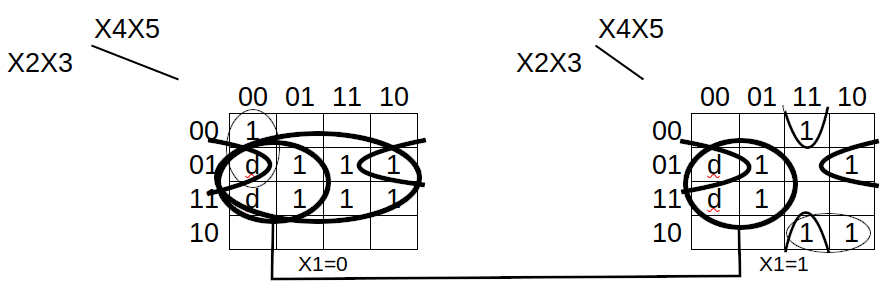
\includegraphics[width=\linewidth]{imgs/mdnf_karno.png}
\end{center}


\begin{equation*}
  \text{Получаем:}\hspace{1.5cm} C_{min}(f)= 
  \begin{Bmatrix}
    0 & X & 1 & X & X \\
    X & X & 1 & 0 & X \\
    X & 0 & 1 & X & 0 \\ 
    0 & 0 & X & 0 & 0 \\ 
    1 & X & 0 & 1 & 1 \\ 
    1 & 1 & 0 & 1 & X 
  \end{Bmatrix}
  \begin{pmatrix}
    1 \\ 2 \\ 3 \\ 4 \\ 5 \\ 6
  \end{pmatrix}
  S^a = 19; \hspace{0.5cm} S^b = 25
\end{equation*}

Отметим, что цены минимальных покрытий, полученных методом Квайна – 
Мак-Класки и с помощью карт Карно, совпадают, так как цена минимального 
покрытия булевой функции не зависит от метода его нахождения \\

МДНФ имеет следующий вид: \\
$ f = \
\nx{1}\x{3} \vee \
\x{3}\nx{4} \vee \
\nx{2}\x{3}\nx{5} \vee \
\nx{1}\nx{2}\nx{4}\nx{5} \vee \
\x{1}\nx{3}\x{4}\x{5}  \vee \
\x{1}\x{2}\nx{3}\x{4} \
$


\subsubsection{Определение МКНФ}

Получение МКНФ производится по нулевому покрытию булевой функции. 
Для этой цели на карте Карно выделяются клетки, соответствующие наборам 
аргументов,  на  которых  функция  принимает  нулевое  значение  (клетки 
отмечаются нулем). \\

\begin{center}
  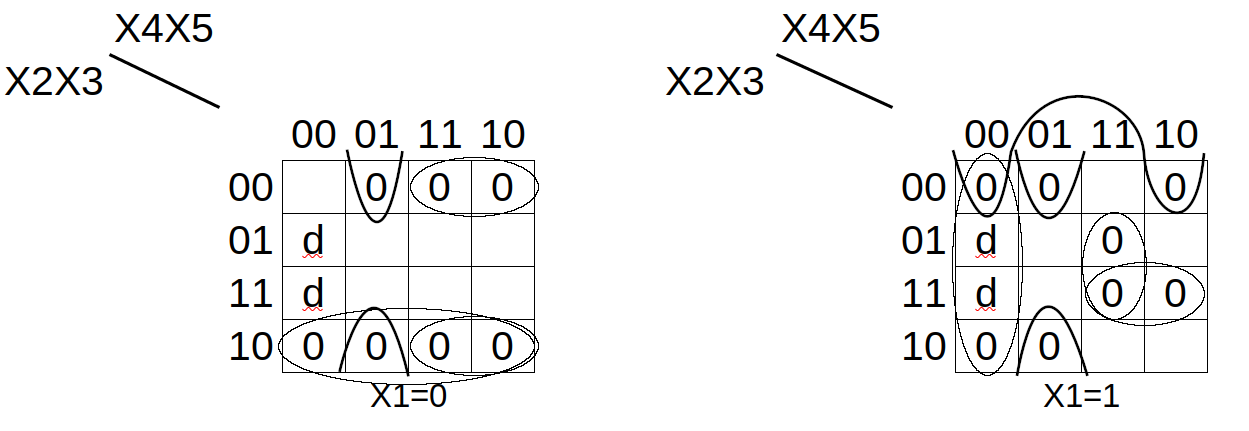
\includegraphics[width=\linewidth]{imgs/mknf_karno.png}
\end{center}

\begin{equation*}
  \text{Получаем:}\hspace{1.5cm} C_{min}(f)= 
  \begin{Bmatrix}
    0& 1& 0& X& X \\
    X& X& 0& 0& 1 \\
    0& X& 0& 1& X \\
    1& X& X& 0& 0 \\
    1& X& 1& 1& 1 \\
    1& 1& 1& 1& X \\
    1& 0& 0& X& 0 
  \end{Bmatrix}
  \begin{pmatrix}
    1 \\ 2 \\ 3 \\ 4 \\ 5 \\ 6
  \end{pmatrix}
  S^a = 24; \hspace{.5cm} S^b = 30
\end{equation*}

МКНФ : $f = \ 
(\x{1} \vee \nx{2} \vee \x{3}) \cdot \
(\x{3} \vee \x{4} \vee \nx{5}) \cdot \
(\x{1} \vee \x{3} \vee \nx{4}) \cdot \
(\nx{1} \vee \x{4} \vee \x{5}) \cdot \
(\nx{1} \vee \nx{3} \vee \nx{4} \vee \nx{5}) \cdot \
(\nx{1} \vee \x{2} \vee \x{3} \vee \x{5})\cdot \
(\nx{1} \vee \nx{2} \vee \nx{3} \vee \nx{4})\
$